\subsection{De Instrucciones a Acciones}

% Se estableció tener un servicio aparte para la ejecución de las ordenes. Esto se debe a las condiciones especiales que debe tener el encargado de realizar el paso final en el ciclo MAPE-K (Ver figura \ref{fig:mapek}). 

% Smart Campus UIS, como plataforma, se ejecuta sobre contenedores de docker; y para efectos de esta primera versión del proyecto, toda la arquitectura de presente, se ejecuta sobre contenedores. Siendo así, la característica principal que debe tener nuestro ejecutor, es la posibilidad de comunicarse con los diferentes contenedores.

% Esto se realizó a partir de 

Ya con las instrucciones necesarias para poder realizar cambios en la arquitectura de las aplicaciones, se realizó la implementación de un servicio encargado de ejecutar las ordenes recibidas desde \textit{Bran}.

Ahora, Smart Campus UIS, como plataforma, se ejecuta sobre contenedores de docker; y para efectos de esta primera versión del proyecto, toda la arquitectura de presente, se ejecuta sobre contenedores. Como consecuencia, era necesario que el servicio implementado, tuviera la de ejecutar comandos de docker con el fin de poder llevar a cabo las acciones.

Esto se solucionó usando la Docker Engine API como el canal de comunicación entre el servicio, y el resto de la arquitectura. Esto se debe a que, esta API REST, permite la interacción directa con el daemon de Docker \cite{docker}, posibilitando la ejecución de todos los comandos relacionados con docker, desde el iniciar y detener servicios hasta crear y eliminar contenedores.

El servicio, apodado \textit{DoThing}, realiza visto en la figura \ref{fig:DoThing}. Este está orientado principalmente al procesamiento de las peticiones realizadas, por lo que es relativamente sencillo en cuanto a las acciones que este realiza. 

\begin{figure}[ht]
    \centering
    \caption{Proceso base de DoThing}
    \label{fig:DoThing}
    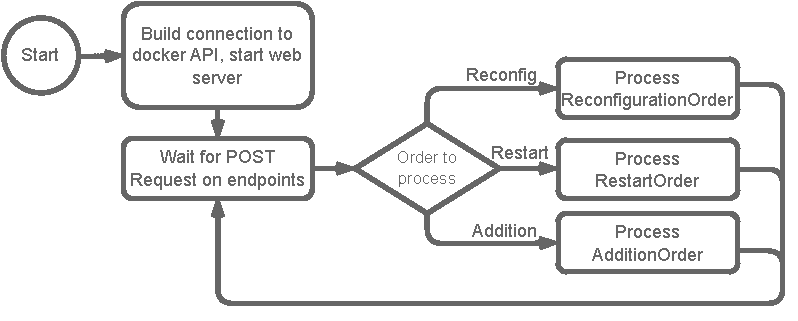
\includegraphics[width=0.75\linewidth]{images/DoThingProcess.pdf}
\end{figure}

Tras inicializar la conexión con la API de Docker, iniciará un servidor web por el cual estará recibiendo las órdenes a ejecutar. Cada tipo de acción tiene su propio endpoint donde se realiza un proceso específico para poder ejecutarla. Cada acción realizada, registrará los contenedores afectados en un registro interno, con el fin de facilitar el procesamiento de múltiples acciones sobre un servicio. 

Las ordenes de \textit{Addition}, como se referencia en la figura \ref{fig:DoThingAddition}, realizan el proceso a partir de la \texttt{image}, \texttt{env\_vars} y \texttt{args}, declarados en la orden, para construir el contenedor con su respectivo servicio.

\begin{figure}[ht]
    \centering
    \caption{Proceso para la ejecución de ordenes de adición}
    \label{fig:DoThingAddition}
    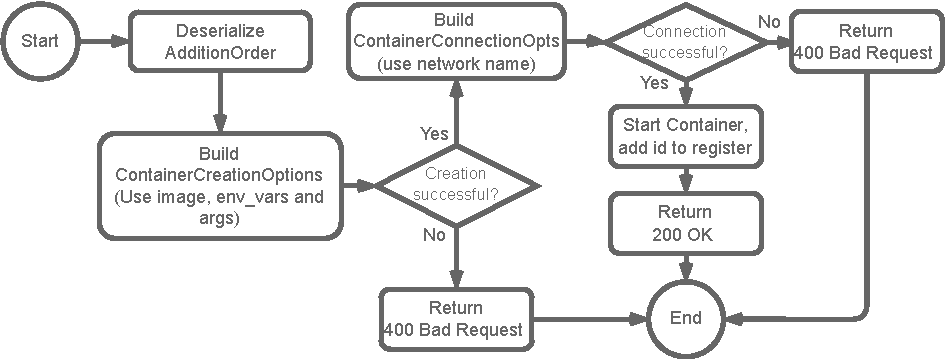
\includegraphics[width=0.8\linewidth]{images/DoThingAddition.pdf}
\end{figure}

Una vez se tenga el contenedor creado, usando \texttt{network\_name}, se conectará el contenedor creado a la red indicada. De no presentarse errores durante este proceso, se iniciará el contenedor, se agrega al registro y retorna \texttt{200 OK}. 

Las órdenes de tipo \textit{Restart}, referenciadas en la figura \ref{fig:DoThingRestart} pueden ejecutarse de una de dos maneras, dependiendo del estado del servicio a afectar. 

\begin{figure}[ht]
    \centering
    \caption{Proceso para la ejecución de ordenes de reinicio}
    \label{fig:DoThingRestart}
    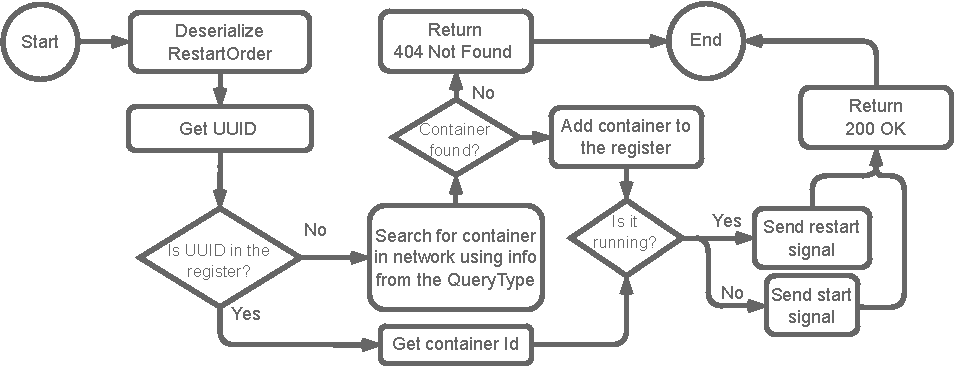
\includegraphics[width=0.9\linewidth]{images/DoThingRestart.pdf}
\end{figure}

Primero, se realiza la búsqueda del contenedor en el registro; de no estar presente, se realizará la búsqueda de este usando la información proveída en el \textit{QueryType} de la orden.

Una vez identificado el servicio, si está corriendo\footnote{Referido en la documentación de \href{https://docs.docker.com/engine/api/v1.43/\#tag/Container/operation/ContainerInspect}{Docker Engine API} como \textit{Running}}, la orden de reinicio será equivalente al comando \texttt{docker restart <container>}, esto con el objetivo de eliminar \textit{cuelgues} en el servicio. Por el contrario, si el contenedor no está en ejecución, la orden ejecutará el equivalente al comando \texttt{docker start <container>}, para así iniciar nuevamente el servicio.

Finalmente, las órdenes de tipo \textit{Reconfigure}, cuyo proceso puede verse en la figura \ref{fig:DoThingReconfig}, es similar al realizado para las órdenes de tipo \textit{Restart}. 

\begin{figure}[ht]
    \centering
    \caption{Proceso para la ejecución de ordenes de reconfiguración}
    \label{fig:DoThingReconfig}
    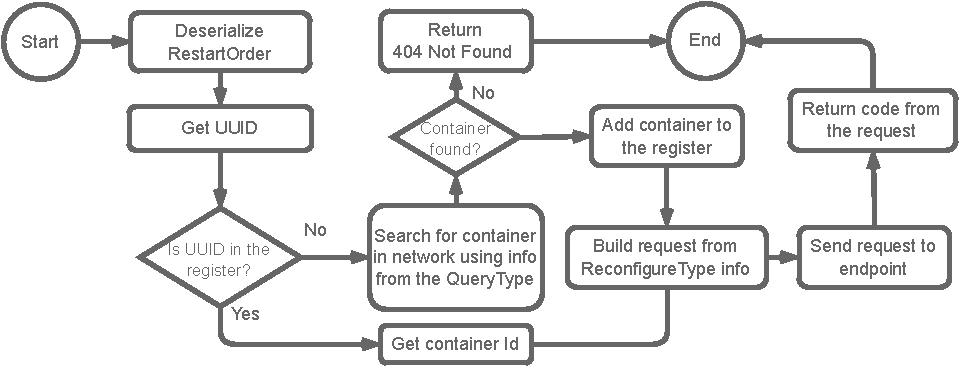
\includegraphics[width=0.8\linewidth]{images/DoThingReconfig.pdf}
\end{figure}

Una vez ubicado el servicio, se construirá, a partir de los datos reportados en \textit{ReconfigureType}, la petición a realizar en el servicio. Esta, en consecuencia, se enviará usando un cliente \textit{Http} y esperará a la respuesta de esta. El resultado, de esta transacción, será el mismo reportado por \textit{DoThing} hacia \textit{Bran}.

Ahora, con la implementación de este servicio, encargado de ejecutar las acciones requeridas para la adaptación de las arquitecturas de las aplicaciones, completa el ciclo autonómico MAPE-K implementado para Smart Campus UIS. 

Una vez ejecutadas las órdenes; el efecto de estas, serían captadas por el observador, evaluando nuevamente el estado de la aplicación, e, idealmente, reportando un cambio positivo hacia la coherencia esperada con el estado de referencia definido en un principio.

La arquitectura final del presente proyecto, con toda la implementación de los servicios, puede ver se en la figura \ref{fig:StarDuckFinal}.


\begin{figure}[ht]
    \centering
    \caption{Arquitectura completa del proyecto}
    \label{fig:StarDuckFinal}
    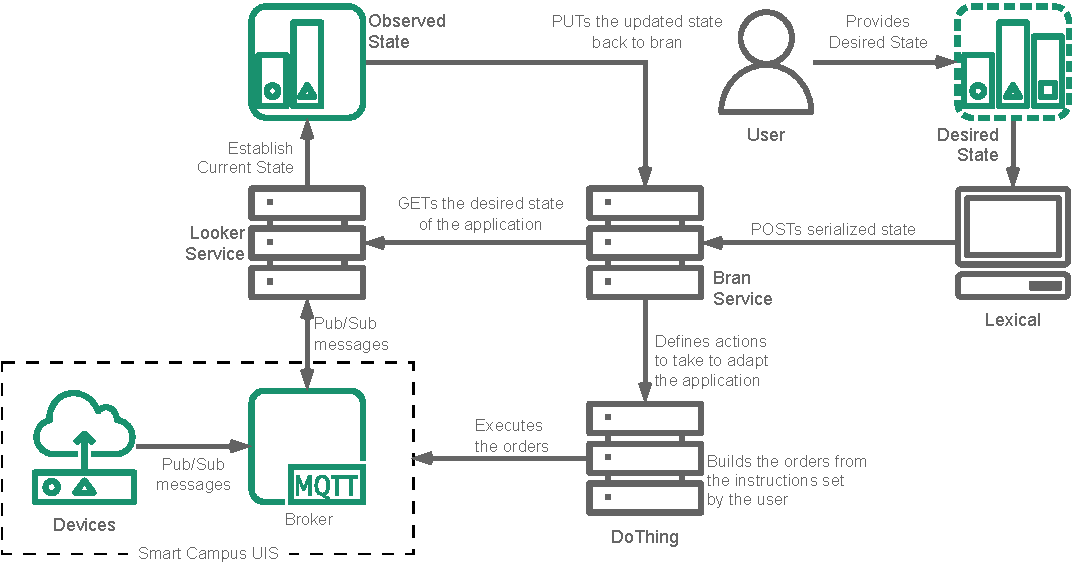
\includegraphics[width=\linewidth]{images/StarDuckFinal.pdf}
\end{figure}